\section{Audio} \label{audio}
Geräusche und Musik im Spiel sind ein wesentlicher Bestand, denn es erhöht die Erlebnisqualität und gibt jedem Spiel einen eigenen Charakter. Geräusche ermöglichen es dem Spieler außerdem zusätzliche Informationen wie beispielsweise die Entfernung und Richtung aus der er einen Gegner erwarten kann, zu erhalten. 

\subsection{Wichtige Komponenten in Unity}
Um Töne in Unity abzuspielen, sind folgende Komponenten notwendig:

\begin{itemize}
	\item \textit{AudioListener}: Komponente, bei der Töne empfangen werden.
	\item \textit{AudioSource}: Komponente, die Töne abspielt. 
\end{itemize}

Damit näher in der Umgebung entstehende Geräusche auch lauter sind als weiter entfernte und der Spieler Geräusche aus einer bestimmten Richtung orten kann, müssen Einstellungen bei jeder \textit{AudioSource} gemacht werden. Durch diese Einstellungen und der Entfernung der \textit{AudioSource} vom \textit{AudioListener} ist es Unity möglich, die Richtung und Lautstärke für die Entfernung des Spielers zum Geräusch genau zu berechnen. Diese Informationen werden dem physikalischen Soundsystem des Spielers mitgeteilt, sodass der Nutzer auch hören kann, aus welcher Richtung das Geräusch entstammt.

Um es dem Benutzer zu ermöglichen Geräusche verschiedener Kategorien, wie beispielsweise die Hintergrundmusik oder die Soundeffekte unterschiedlich einzustellen, werden sogenannte \textit{AudioMixer} und \textit{AudioMixerGroups} benötigt. Abbildung \ref{fig:audio_routing} zeigt das Zusammenspiel dieser Komponenten für den aktuellen Projektstand.

\begin {figure}[h]
	\begin {center}
	    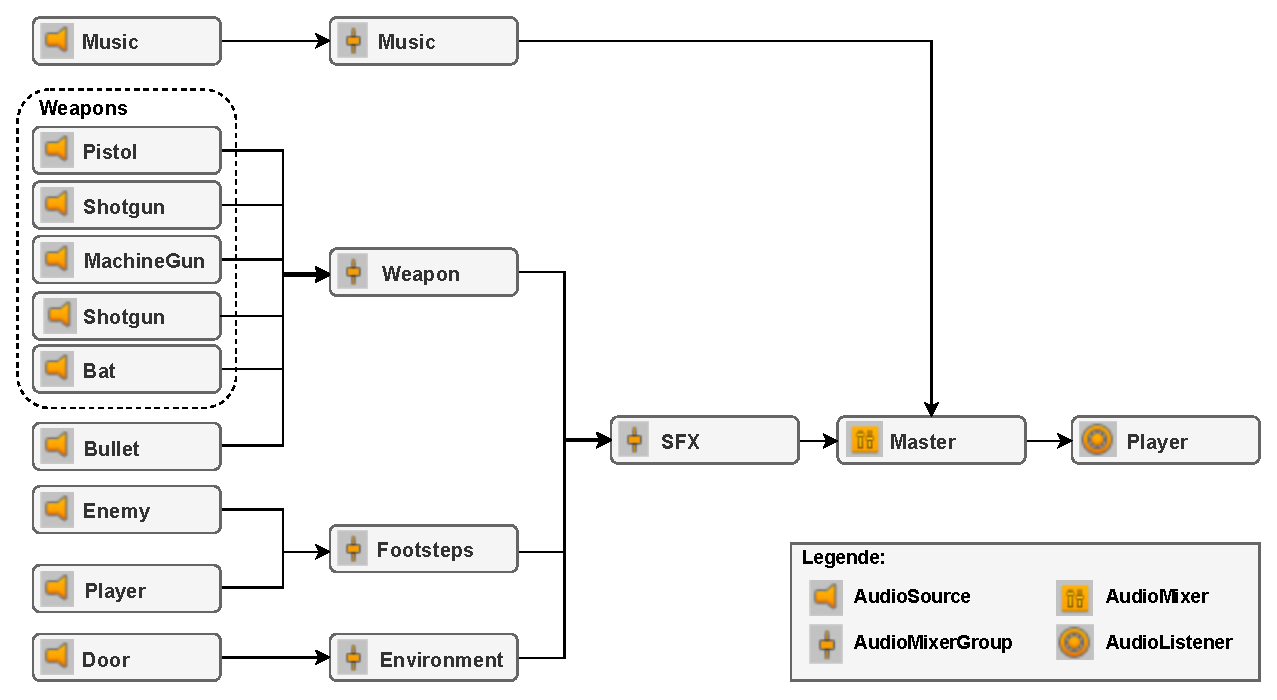
\includegraphics[width=1\textwidth]{pics/audio_routing.eps}
		\caption{Weiterleitung der Audiosignale}
		\label{fig:audio_routing}
	\end {center}
\end {figure}

Falls keine \textit{AudioMixer} und AudioMixerGruppen (\textit{AudioMixerGroups}) eingestellt sind, werden Töne direkt von der \textit{AudioSource} zum \textit{AudioListener} geleitet. Für jede \textit{AudioSource} kann eingestellt werden, zu welcher \textit{AudioMixerGroup} diese die Töne weiterleiten soll. Für einen \textit{AudioMixer} können dabei beliebig viele AudioMixerGruppen eingerichtet werden. Durch eine Hierarchie kann festgelegt werden, zu welcher übergeordneten AudioMixerGruppe eine bestimmte \textit{AudioMixerGroup} empfangene Töne weiterleitet. Standardmäßig existiert bereits bei Erstellung eines \textit{AudioMixers} eine \textit{AudioMixerGroup}: Der \textit{Master}. Da alle Tonsignale des \textit{AudioMixers} an diese Gruppe weitergeleitet werden, kontrolliert diese die Gesamtlautstärke. Ist für einen \textit{AudioListener} ein \textit{AudioMixer} eingestellt, so leitet die \textit{Master}-Gruppe eines \textit{AudioMixers} die Tonsignale an diesen weiter.
 
\subsection{Das Audiosystem}\label{sec:audiosystem}
Damit ein Spieler hören kann, wie weit ein Gegner entfernt ist und aus welcher Richtung er kommt, müssen folglich die Töne von Gegnern immer genau dort entstehen, wo sich die Gegner gerade befinden. Daher muss jeder Gegner eine eigene Audioquelle besitzen.

Damit eine Audioquelle (\textit{AudioSource}) Töne abspielen kann, muss ihr diese sogenannte Tonspur (\textit{AudioClip}) übergeben und die Methode \texttt{Play()} der Audioquelle aufgerufen werden. Die im Projekt verwendeten \textit{AudioClips}\cite{KompositeSoundCaesarBostonProfiDevelopers.2019} sind vom \textit{Asset Store}\cite{Unity_Doc_Assets_Bib} importiert worden. Zu jeder Tonspur gibt es Eigenschaften wie beispielsweise die Lautstärke, die \textit{AudioMixerGroup}, an die die Tonsignale weitergeleitet werden sollen oder, ob der \textit{AudioClip} in einer Endlosschleife gespielt werden soll. All diese Eigenschaften werden zusammen mit dem \textit{AudioClip} in einer eigenen Klasse \texttt{Sound}\ref{fig:audio_system} gespeichert. Neben Eigenschaften, die jeder \textit{AudioClip} besitzt, gibt es zwei verschiedene Situationen, in denen Geräusche entstehen und somit eine Unterteilung in zwei verschiedene Kategorien erforderlich machen: 

\begin{enumerate}
	\item Die Töne entstehen an bestimmten Orten im Spiel.
	\item Es gibt keinen bestimmten Ort im Spiel, von dem aus die Tonspur abgespielt wird.
\end{enumerate}

Die mit Abstand meisten Tonspuren müssen an bestimmten Orten abgespielt werden. Wird beispielsweise eine Waffe abgefeuert, so entsteht ein hörbares Geräusch genau bei der Waffe, ein Geräusch während dem Fliegen der Kugel und ein weiteres Geräusch genau bei dem Einschlagspunkt des Geschosses. Für das Spiel wurde zweiteres weggelassen, da zu viele Geräusche ein Spieler als störend empfinden würde, dieses im Spiel klar zu sehen ist und somit keine zusätzlichen Informationen liefert. Zudem muss beachtet werden, dass eine bestimmte Waffe im Spiel mehrfach vorhanden sein, von unterschiedlichen Positionen aus zeitlich versetzt voneinander abgefeuert werden kann, mehrere Geschosse des gleichen Typs zur gleichen Zeit existieren und auch zeitlich als auch örtlich unterschiedliche Einschlagspunkte haben können. Zu diesen Tonspuren müssen weitere Eigenschaften definiert werden, die es dem Spieler ermöglichen sowohl die Richtung als auch die Nähe von entstehenden Geräuschen einschätzen zu können.

Zum zweiten Fall gehört beispielsweise die Hintergrundmusik. All die Fälle, die zu dieser Gruppe gehören, haben zudem die Eigenschaft, dass die gleiche Tonspur nie gleichzeitig abgespielt wird. Denn der Spieler würde dies als störend empfinden. Somit kann jede Tonspur in dieser Gruppe einer einzelnen Audioquelle zugeordnet werden.

Da die Tonspuren für diese zwei Fälle unterschiedliche zusätzliche Eigenschaften benötigen, wurde eine Klasse \texttt{DynamicSound} für örtlich positionierte und eine andere Klasse \texttt{StaticSound} für synchron und ohne bestimmten Ort abzuspielende Tonspuren entworfen. Diese erben von der abstrakten Klasse \texttt{Sound}. 

Um in Unity verwendet werden zu können, muss nun zunächst für jede Tonspur eine Instanz einer der beiden Klassen erstellt und die Eigenschaften für die Tonspuren individuell angepasst werden. Dies muss möglich sein, da die Tonspuren bereits bei Erstellung unterschiedliche Lautstärken haben können. Ein sehr großer Vorteil, der sich daraus ergibt ist, dass die gleiche Tonspur für mehrere Situationen verwendet werden und somit der Entwicklungsaufwand deutliche reduziert werden kann. Wird beispielsweise eine schallgedämpfte Pistole implementiert, so kann die Tonspur der Pistole wiederverwendet und vor allem die Lautstärke dieser Tonspur und anderer Eigenschaften verändert werden. Diese eingestellten Sound-Objekte dienen dazu im Spiel Audioquellen von Spielobjekten zu konfigurieren und werden daher im nachfolgenden als \glqq{Konfigurationsobjekte\grqq{} bezeichnet.

\subsubsection{Designmöglichkeiten}
Die zentrale Rolle des zu entwerfenden Audiosystems ist es nun, diese Konfigurationsobjekte zu verwalten. Grundsätzlich gibt es hierfür zwei Implementierungsmöglichkeiten:

\begin{itemize}
	\item Eine zentrale Klasse verwaltet alle Konfigurationsobjekte und übergibt auf Anfrage eine Referenz auf das angefragte Objekt.
	\item Jedes \textit{Prefab} verwaltet die zu es gehörenden Konfigurationsobjekte.
\end{itemize}

In Unity ist es üblich solche bereits vor Laufzeit vorhandenen Objekte in einer Liste zu speichern. Alle Konfigurationsobjekte in einer zentralen Klasse in einer Liste zu speichern, würde dazu führen, dass diese schnell anwächst und somit zu folgenden Problemen:

\begin{enumerate}
	\item Änderungen an Einstellungen der Konfigurationsobjekte sind schlecht durchführbar, da das richtige Konfigurationsobjekt erst unter allen in der Liste gespeicherten Objekten gesucht werden muss. 
	\item Um eine Tonspur abzuspielen, muss immer unter allen existierenden Konfigurationsobjekten gesucht werden. Mit der Häufigkeit des Abspielens von Geräuschen ist dies ein bedeutender Faktor. 
	\item Im Code muss für jedes machbare Geräusch eines Spielobjektes speziell das dazugehörige Konfigurationsobjekt zum Abspielen angegeben werden. Da die zentrale Komponente alle Sounddateien besitzt, kann sie beispielsweise mit dem Befehl \glqq{}Waffe abfeuern\grqq{} nicht genau zuordnen, ob die Tonspur von dem Maschinengewehr oder der Pistole abgespielt werden soll.
\end{enumerate}

Durch eine geeignete Datenstruktur kann der Aufwand zum Suchen des richtigen Konfigurationsobjektes verringert werden. Dennoch ist dieser Aufwand größer, als wenn jedes \textit{Prefab} bereits die Konfigurationsobjekte besitzt, die es benötigt. 

\begin{itemize}
	\item Dadurch muss nur unter den für das Spielobjekt benötigten Konfigurationsobjekte gesucht werden, um das richtige Objekt zu finden. 
	\item Da beispielsweise eine Schrotflinte ihre eigenen charakteristischen Geräusche für das Abfeuern der Waffe oder das Nachladen besitzt, muss das zugehörige in Unity verwendete \textit{Prefab} auch seine eignen charakteristischen Geräusche besitzen können. Das Beibehalten dieser Zuordnung wird durch diesen Ansatz bewahrt, wodurch die Tonspuren leicht konfigurierbar und erweiterbar sind.
\end{itemize} 

Es wird darauf hingewiesen, dass jede Tonspur nur einmal physikalisch im Projekt existiert. Die zu den Spielobjekten  zugehörigen Audioquellen erhalten lediglich eine Referenz auf die Tonspur. Mit der Konfiguration der Audioquelle durch die Eigenschaften der Tonspur ist Unity in der Lage die für das physikalische Audiosystem des Spielers notwendigen Audiosignale zu generieren. %TODO: Hier wäre gut zu erklären, wie Unity die Tonstreifen intern behandelt. Werden diese intern repliziert, um die gleichzeitig abspielen zu können?


\subsubsection{Die Implementierung}
\begin {figure}[h]
	\begin {center}
	    \includegraphics[width=1\textwidth]{pics/audio_audiosystem.pdf}
		\caption{Das Audio-System}
		\label{fig:audio_system}
	\end {center}
\end {figure}
Aus den vorangegangenen Überlegungen wurde das in Abbildung \ref{fig:audio_system} zu sehende Klassendiagramm für das Audiosystem entworfen und implementiert. Dabei wurden die einem \textit{Prefab} zuordnungsbaren Konfigurationsobjekte in eine eigene Komponente ausgelagert und an das Spielobjekt des \textit{Prefabs} gebunden. Dadurch entsteht keine direkte Zuordnung zwischen der Klasse und der Audiokomponente. Die Klasse muss nur auf die Basisklasse \textit{AudioComponent} zugreifen und die Methode \texttt{Play(...)} aufrufen. Durch Vererbung kann dazu diese Methode an bestimmte Typen wie Geschosse, Waffen oder Gegnern und Spielern angepasst werden. Dies ermöglicht es auch im Code nicht spezifizieren zu müssen, welche Tonspur von welcher Waffe genau abgespielt werden soll. Es reicht der Komponente mitzuteilen, dass die Tonspur zum Abfeuern der Waffe abgespielt werden soll. Dadurch sind die Abhängigkeiten im Code zur Audiokomponente geringer als bei Verwendung einer zentralen Instanz.

\subsection{Gegner reagieren auf Geräusche} \label{sec:gegnerreaktionaufaudio}
Im Spiel sollen Geräusche, die der Spieler verursacht einen Gegner auf diesen aufmerksam machen können, sodass der Gegner den Spieler gegebenenfalls sucht und bei Sichtkontakt angreift. 

\subsubsection{Designmöglichkeiten}
Es gibt grundsätzlich zwei Möglichkeiten der Umsetzung:
\begin{enumerate}
	\item Gegner prüfen in regelmäßigen Abständen auf Geräusche in der näheren Umgebung.
	\item Geräusche benachrichtigen Gegner in der näheren Umgebung.
\end{enumerate}

Der erstere Ansatz würde dazu führen, dass für den Spieler unverständliche Effekte auftreten könnten wie beispielsweise, dass die Aufmerksamkeitsanzeige eines Gegners bei einem vom Spieler verursachten sehr lauten Geräusch in seiner näheren Umgebung entweder gar nicht oder sofort stark ansteigt. Dies liegt daran, dass ein Radius um den Gegner herum bestimmen würde, ob ein Geräusch erkannt werden kann oder nicht. Wie laut das Geräusch dabei ist, spielt zunächst keine Rolle. Würde man versuchen alle möglichen Geräusche miteinzubeziehen, die die Aufmerksamkeit des Gegners erhöhen könnten, so müsste man den Radius auf das lauteste Geräusch setzen, das der Gegner hören könnte. Wird dies umgesetzt, so würden auch sehr viele leisere Geräusche zunächst dabei sein, die nach der Berechnung für die Reichweite der Lautstärke und dem Vergleich der Distanz zum Gegner wieder aussortiert werden. %Die bei dieser Variante resultierende Überlegung ist einen fließenden Übergang durch mehrere Bereiche um den Gegner herum nachzuahmen. Dieser fließende Übergang ist bei letzterer Variante bereits vorhanden: 
Diese unnötige Berechnung ist bei letzterer Variante nicht vorhanden: Dadurch, dass einem Geräusch eine Lautstärke  als Attribut gegeben werden kann, kann auch der Radius für jedes Geräusch, in dem es Gegner aufmerksam macht, flexibel eingestellt werden.   

Daneben muss unterschieden werden, ob der Spieler oder der Gegner das Geräusch verursacht hat. Dabei wurde festgelegt, dass für Waffen und Projektile egal ist, ob ein Spieler oder ein Gegner die zugehörigen Geräusche verursacht hat, da ein Gegner seine Waffe nicht einsetzen würde, wenn ein Spieler nicht in der näheren Umgebung wäre. Durch Vererbung kann bei der zweiten Variante vermieden werden, dass die Funktion für die Benachrichtigung über ein Geräusch aufgerufen wird, indem nur die Methoden \texttt{Play(...)} der Audiokomponenten von Waffen, Geschossen und Spielern diese Funktionalität aufrufen. Bei der ersteren Version muss hingegen eine Überprüfung zwingend stattfinden.

Als nächstes muss die durch diese Funktionalität  entstehende unvermeidbare Auslastung für die zusätzlichen Berechnungen berücksichtigt werden. Beim ersteren Ansatz steigt die Auslastung pro Gegner im Spiel an, da jeder Gegner andauernd prüfen muss, ob Geräusche auf einen Spieler in der Nähe Rückschlüsse ziehen lassen. Geräusche außerhalb der Aufmerksamkeitsreichweite der Gegner erhöhen hingegen nicht die Auslastung zusätzlich. Beim letzteren Ansatz verursacht potentiell jedes aktive Geräusch eine höhere Auslastung, da überprüft werden muss, ob ein Gegner in Reichweite ist. Gegner außerhalb der Reichweite der Geräuschlautstärke hingegen erhöhen die Auslastung nicht.

Die Auslastung bei beiden Varianten kann dabei auf ein Minimum reduziert werden, indem nur in einem gewissen Umkreis um den Spieler herum die zugehörigen Funktionen aufgerufen werden, wodurch beide Varianten in etwa die gleiche Auslastung verursachen sollten. Für das Spiel wurde die letztere Variante implementiert, da diese für den Spieler ein verständlicheres Verhalten von Gegnern zur Folge hat und bereits ohne größere Performanzeverbesserung gute Resultate liefert.

\subsubsection{Die Implementierung}
Für die Implementierung dieses Features kann auf das Konzept des Audiosystems zurückgegriffen werden. Dabei muss jedes mal, wenn die Methode \texttt{Play(...)} einer Audiokomponente eines Spielers, eines Geschosses oder einer Waffe aufgerufen wird überprüft werden, ob sich Gegner in der Umgebung befinden. Hierfür kann die Vererbung genutzt werden, um diese Überprüfung bei Geräuschen ausgehend von Gegnern zu vermeiden. Da jedes Geräusch eine unterschiedliche Lautstärke hat und auch die Entfernung sowie die Art des Gegners eine Rolle spielen kann, wie sehr die Aufmerksamkeit eines Gegners ansteigt, müssen diese bei der Berechnung für die Aufmerksamkeitserhöhung miteinbezogen werden. Hierfür besitzt jeder Gegner ein eigenes Attribut wie sehr die Aufmerksamkeit von diesem erhöht wird, jedes Objekt des Typs \texttt{DynamicSound} besitzt ein Attribut für die Aufmerksamkeitserhöhung und die Strecke zwischen dem Ursprungsort des Geräusches und der aktuellen Position des Gegners kann durch die zwischen diesen Positionen liegende Wegstrecke berechnet werden. Dabei wird nicht die Luftstrecke, sondern die hindernisfreie Wegstrecke des Geräusches bis zum Gegner für die Berechnung herangezogen. Für die Berechnung wird die Funktion \texttt{GetAwarenessIncrease(...)} genutzt. Dabei wird vor der Berechnung zunächst mit der Methode \texttt{GetEnemiesInRange(...)} die in der Nähe befindlichen Gegner gesucht. Sind keine Gegner in dem Wirkungsbereich des Geräusches, so wird die Methode verlassen.

\subsection{Einstellung der Lautstärke verschiedener Kategorien}
\begin {figure}[h]
	\begin {center}
	    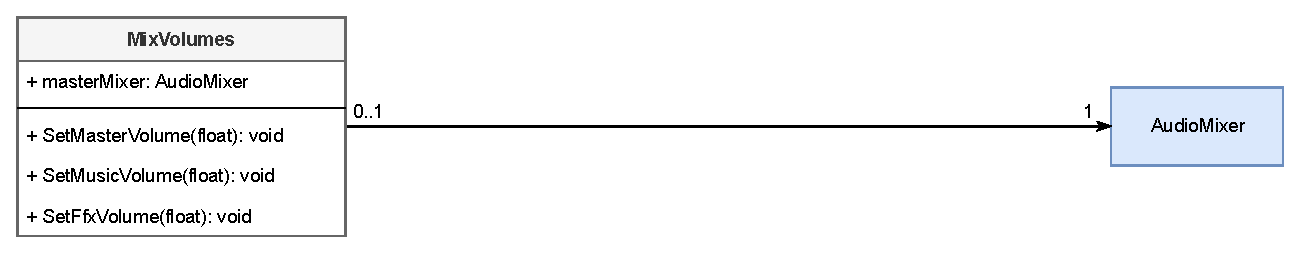
\includegraphics[width=1\textwidth]{pics/audio_category_configuration.eps}
		\caption{Implementierung für das Einstellen der Lautstärke verschiedener Kategorien}
		\label{fig:audio_category_configuration}
	\end {center}
\end {figure}
Für einen Benutzer ist es beim Audiosystem wichtig einstellen zu können, wie laut die Lautstärke jeder einzelnen Soundkategorie ist. Abbildung \ref{fig:audio_category_configuration} zeigt den hierfür implementierten Teil des Audiosystem. Aktuell kann im Optionsmenü des Hauptmenüs eingestellt werden, wie laut das Gesamtvolumen, die Hintergrundmusik und die Soundeffekte sein sollen. Das Audiosystem wurde auch in diesem Bereich so ausgelegt, dass weitere Kategorien leicht implementiert werden können. Bei jedem Schieberegler für diese Einstellungen wird bei Veränderung der Position dieses Reglers ein Event ausgelöst welches eine bestimmte Funktion in der Klasse \texttt{MixVolumes} anspricht mit dem aktuellen Stand des Reglers von null bis eins.




